\chapter{Energy Reconstruction}
\label{sec:energy}
	The second stage is the reconstruction of the particle's energy using a~fit of its reconstructed track (see \cref{sec:track}). We have tested three ways of reconstructing the energy. Fitting is done using the MINUIT algorithm implemented in ROOT~\cite{ROOT}.
	
	The \textbf{Cubic Spline Fit} was a~tested and later rejected method of energy reconstruction. It uses smoothly connected piecewise cubic polynomials between uniformly spaced nodes. The reconstructed energy is calculated from the fit parameters by computing the radius of curvature at different points of the fitted curve using the known magnitude of the magnetic field perpendicular to the trajectory. We rejected this method because the tuning of the fit turned out to be unpractical compared to the other used methods.
	
	The \textbf{Circle and Lines Fit} was chosen as an alternative since this corresponds to the shape of a~trajectory of a~charged particle crossing a~finite volume with a~homogeneous magnetic field. The energy of the particle can be estimated using the fitted radius and the magnitude of the perpendicular magnetic field in the middle of the \ac{OFTPC}.
	
	The \textbf{Runge-Kutta Fit} uses the 4th order Runge-Kutta numerical integration described in \cref{sec:rks}. Initial parameters of the track (including the particle's energy) are optimized so that the integrated trajectory fits to the reconstructed one. This fit can also be performed as a~single parameter (energy) fit if we get the initial position and orientation of the particle on the entrance to the \ac{OFTPC} from previous detectors (\ac{TPX3} and \ac{MWPC}, see \cref{sec:IEAP}).
	
	\section{Cubic Spline Fit}
	\label{sec:cspline}
		The first method for the estimation of the kinetic energy of the particle uses a~cubic spline fit. We use an electron track simulated using the microscopic simulation, described in detail in \cref{sec:microfirst}. The track was reconstructed using the map described in \cref{sec:map}.
				
		In order to calculate the spline, we use the class \texttt{TSpline3} from ROOT. This allows us to evaluate the spline using the coordinates $(x_n,z_n)$ of each node and the derivatives $d_1,d_2$ in the first and the last node. We can fit these parameters of a~fixed amount of nodes to the simulated trajectory. We use the IMPROVE algorithm provided by the \texttt{TMinuit} class in ROOT. This algorithm attempts to find a~better local minimum of the minimized function after converging.
		
		After the fit converges, we calculate an energy estimate using the radius of curvature, which we can extract from the fitted spline equation at every point of the trajectory. The part of the spline corresponding to a~given node is defined as
			\begin{equation}
				z(x) = z_n + b \Delta x+c(\Delta x)^2+d(\Delta x)^3,
			\end{equation}
		where $\Delta x = x-x_n$ and $b,c,d$ are coefficients. Using this equation, we derive the radius of curvature\footnote{For the general formula see \url{https://en.wikipedia.org/wiki/Curvature\#Graph_of_a_function}.} as:
			\begin{equation}
				r(x) = \frac{\left(1+z'^2(x)\right)^\frac{3}{2}}{z''(x)} = \frac{\left(1+\left(b+2c\Delta x+3d(\Delta x)^2\right)^2\right)^\frac{3}{2}}{2c+6d\Delta x}.
			\end{equation}
		Based on the geometry of our~detector, we assume that the magnetic field satisfies $\mathbf{B}(x,0,z) = (0,B(x,z),0)$ for a~track in the XZ~plane. Since the electron is relativistic, the effect of the electric field on its trajectory is negligible. The Lorentz force $\mathbf{F}_\text{L}$ is then always perpendicular to the momentum of the electron and acts as a~centripetal force $\mathbf{F}_\text{c}$:
			\begin{gather}
				\begin{aligned}
					\mathbf{F}_\text{L} &= \mathbf{F}_\text{c},\\
					\norm{e\mathbf{v}\times\mathbf{B}} &= \frac{\gamma m_e v^2}{r},\\
					e c\beta B &= \frac{E_{0e} \beta^2}{r\sqrt{1-\beta^2}},\\
					\sqrt{1-\beta^2} &= \frac{E_{0e} \beta}{ecBr},
				\end{aligned}\\
				\beta^2(x) = \left[1+\left(\frac{E_{0e}}{ecB(x,z(x))r(x)}\right)^2\right]^{-1}, \label{eq:ekin1}
			\end{gather}
		where $e$~is the elementary charge, $c$~is the speed of light in vacuum, $m_e$~is the rest mass of electron, $E_{0e} = m_e c^2$ is its rest energy, $\gamma$~is the Lorentz factor, $\mathbf{v}$~is the velocity of the electron, and $\beta = \frac{v}{c}$. The kinetic energy for a~given point on the trajectory is then given as
			\begin{equation}
				\label{eq:ekin2}
				E_\text{kin}(x) = \left(\frac{1}{\sqrt{1-\beta^2(x)}}-1\right)E_{0e}.
			\end{equation}
		We could then average these estimates at multiple points (possibly using some weights to account for the change in accuracy) to get a~single value. An example of the reconstruction for a~reconstructed track is shown in \cref{fig:spline}. This method was later rejected in favor of the circle-and-lines fit described in the next section.
		
		\begin{figure}
			\centering
			\begin{subfigure}[t]{0.48\textwidth}
				\centering
				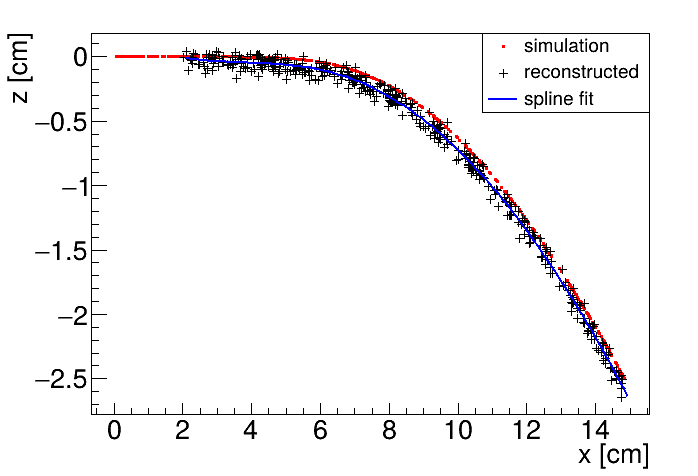
\includegraphics[width=\textwidth]{spline_fit.png}
				\caption{Spline fit of a~reconstructed track.}
			\end{subfigure}
			\hfill
			\begin{subfigure}[t]{0.48\textwidth}
				\centering
				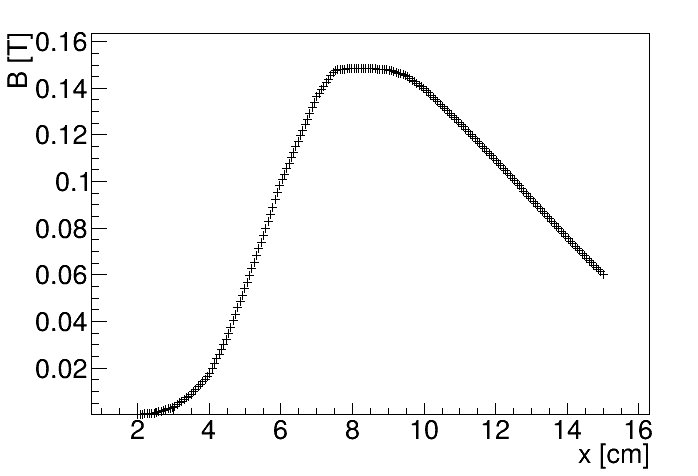
\includegraphics[width=\textwidth]{spline_mag.png}
				\caption{Magnetic field along the track.}
			\end{subfigure}
			\begin{subfigure}[t]{0.48\textwidth}
				\centering
				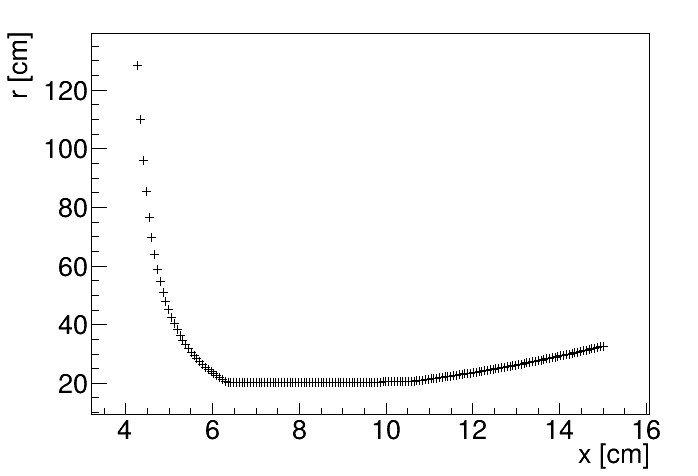
\includegraphics[width=\textwidth]{spline_radius.png}
				\caption{Reconstructed radius of curvature along the track.}
			\end{subfigure}
			\hfill
			\begin{subfigure}[t]{0.48\textwidth}
				\centering
				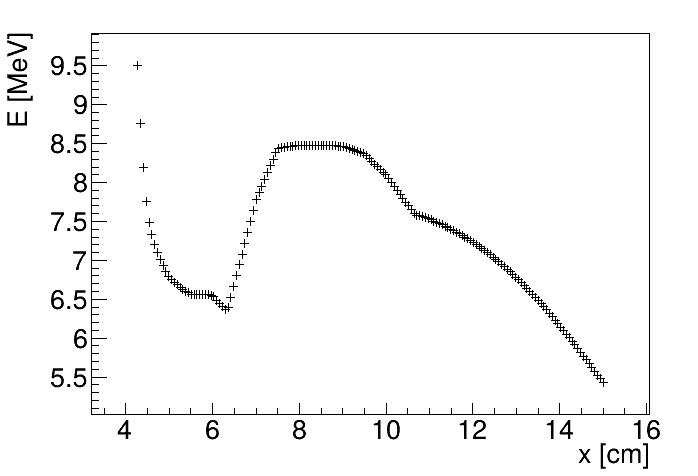
\includegraphics[width=\textwidth]{spline_energy.png}
				\caption{Reconstructed energy along the track.}
			\end{subfigure}
			\caption{Energy reconstruction of a~\qty{7.51}{\MeV} track in a~70:30 Ar:CO$_2$ gas mixture (described in detail in \cref{sec:microfirst}) using a~cubic spline fit with four evenly spaced nodes of points reconstructed using the map.}
			\label{fig:spline}
		\end{figure}
	
	\section{Circle and Lines Fit}
	\label{sec:clines}
		Another way to estimate the particle's kinetic energy is to~fit its trajectory with a~circular arc with lines attached smoothly. This shape of trajectory corresponds to a~movement of a~charged particle through a~homogeneous magnetic field perpendicular to the particle's momentum and limited to a~certain volume. In general, the shape of such a~trajectory with a~non-perpendicularly oriented momentum is a~spiral. In our case, the magnetic field is approximately toroidal and the particle motion is nearly perpendicular to it. At first, we tested a~2D version of this fit, then we adapted it to 3D.
		
		The field in our detector is not homogeneous, it is therefore not entirely clear what value of magnetic field should be used along with the fitted radius (using \cref{eq:ekin1,eq:ekin2}) to get the best estimate for the kinetic energy. Since we only use this method as the first iteration of the particle's energy that we later refine, an optimal solution of this problem is not required. Instead, we tested two options: taking the value of the field in the point, where the track crosses the middle $x$\nobreakdash-coordinate of the \ac{OFTPC}, and taking the average field along it.
		
		\subsection{Two-dimensional fit}
			In the 2D case, the fitted function used for the electron track\footnote{Electron tracks bend towards negative~$z$, we need to use the upper part of the circle.} described in \cref{sec:microfirst} is defined as follows:
				\begin{equation}
					\label{eq:clines2d}
					z(x) = \begin{cases}
								a_1x+b_1 & x<x_1\\
								z_0+\sqrt{r^2-(x-x_0)^2} & x_1\leq x\leq x_2\\
								a_2x+b_2 & x>x_2
						   \end{cases},
				\end{equation}
			where $a_{1,2}$ and $b_{1,2}$ are the parameters of the lines, $(x_0,z_0)$ is the center of the circle, $r$ is its radius, and $(x_{1,2},z_{1,2})$ are the coordinates of the function's nodes. That means we have 9~parameters ($z_{1,2}$ are not used in the function) along with 2~continuity conditions and 2~smoothness conditions. For the fit, we use the coordinates of the nodes and the radius of the circle, which gives us 5~\emph{independent} parameters (only the radius has to be larger than half of the distance between nodes). The continuity conditions (combined with the relations for $z_{1,2}$) are
				\begin{equation}
					\label{eq:ccont}
					z_{1,2} = a_{1,2}x_{1,2}+b_{1,2} = z_0-\sqrt{r^2-(x_{1,2}-x_0)^2},
				\end{equation}
			the smoothness conditions are
				\begin{equation}
					\label{eq:a12}
					a_{1,2} = \frac{x_0-x_{1,2}}{\sqrt{r^2-(x_{1,2}-x_0)^2}}.
				\end{equation}
			Together with \cref{eq:ccont} we get the values of $b_{1,2}$
				\begin{equation}
					\label{eq:b12}
					b_{1,2} = z_{1,2} - a_{1,2} x_{1,2}.
				\end{equation}
			For the coordinates of the center of the circle, we can use the fact that the center has to lie on the axis of its chord. In other words, there is a~value of a~parameter~$t$ such that, using the parametric equation of the axis
				\begin{equation}
					\begin{pmatrix} x_0\\ z_0 \end{pmatrix} = \begin{pmatrix} \frac{x_1+x_2}{2}\\ \frac{z_1+z_2}{2} \end{pmatrix} + t \begin{pmatrix} \frac{z_2-z_1}{2}\\ \frac{x_1-x_2}{2} \end{pmatrix}.
				\end{equation}
			At the same time, the center has to be in a~distance of $r$ from the nodes:
				\begin{gather}
					(x_1-x_0)^2 + (z_1-z_0)^2 = r^2,\notag\\
					\left(\frac{x_1-x_2}{2}+\frac{z_1-z_2}{2}t\right)^2 + \left(\frac{z_1-z_2}{2}+\frac{x_2-x_1}{2}t\right)^2 = r^2,\notag\\
					\left(\left(\frac{x_2-x_1}{2}\right)^2+\left(\frac{z_2-z_1}{2}\right)^2\right)t^2+\left(\frac{x_2-x_1}{2}\right)^2+\left(\frac{z_2-z_1}{2}\right)^2-r^2=0.
				\end{gather}
			Since our electron track bends towards negative $z$ and $x_2 > x_1$, we only care about the solution with $t>0$
				\begin{gather}
					t = \sqrt{\frac{r^2}{\left(\frac{x_2-x_1}{2}\right)^2+\left(\frac{z_2-z_1}{2}\right)^2}-1},\\
					\begin{aligned}
						x_0 = \frac{x_1+x_2}{2} + \frac{z_2-z_1}{2} \sqrt{\frac{r^2}{\left(\frac{x_2-x_1}{2}\right)^2+\left(\frac{z_2-z_1}{2}\right)^2}-1},\label{eq:xz0}\\
						z_0 = \frac{z_1+z_2}{2} - \frac{x_2-x_1}{2} \sqrt{\frac{r^2}{\left(\frac{x_2-x_1}{2}\right)^2+\left(\frac{z_2-z_1}{2}\right)^2}-1}.
					\end{aligned}
				\end{gather}
			The function defined in \cref{eq:clines2d} along with \cref{eq:a12,eq:b12,eq:xz0} derived using the continuity and smoothness conditions (combined with the relations for $z_{1,2}$) fully define our fitted function with parameters $r,x_{1,2},z_{1,2}$.
			
			For the calculation of kinetic energy from the radius of the circle, we use the value of the magnetic field in the middle of the \ac{OFTPC}. An example of a~fit of vertices reconstructed with the map is shown in \cref{fig:circle2d}.
			
			\begin{figure}
				\centering
				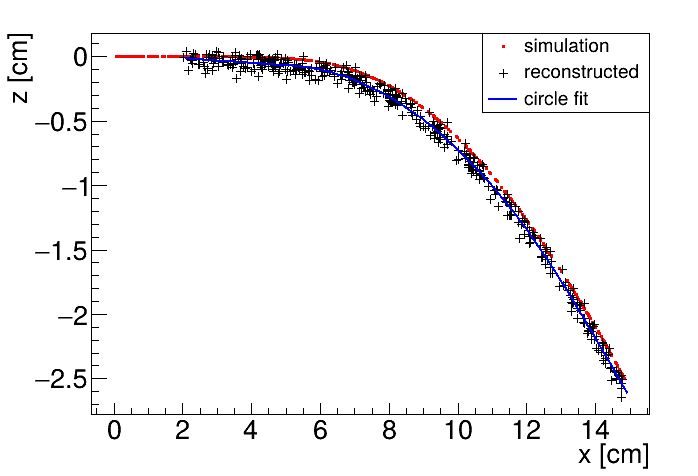
\includegraphics[width=0.48\textwidth]{circ2d_fit.png}
				\hfill
				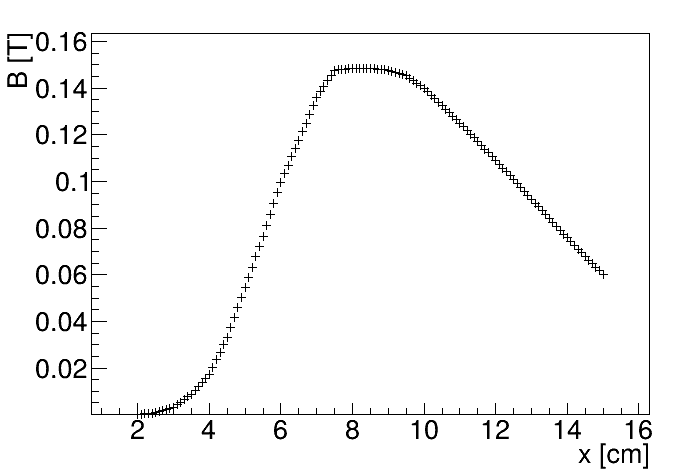
\includegraphics[width=0.48\textwidth]{circ2d_mag.png}
				\caption{Circle-and-lines 2D energy reconstruction of a~\qty{7.51}{\MeV} track in a~70:30 Ar:CO$_2$ gas mixture (described in detail in \cref{sec:microfirst}) reconstructed with the map. The fitted position of the nodes is $(x_1,z_1) = (5.20,-0.07)\,\unit{\cm}$ and $(x_2,z_2) = (14.43,-1.93)\,\unit{\cm}$, the radius is $r = \qty{20.79}{\cm}$. The resulting energy is \qty{7.70}{\MeV}, the magnetic field along the track is shown on the right.}
				\label{fig:circle2d}
			\end{figure}
		
		\subsection{Three-dimensional fit}
			In three dimensions, the shape of a~trajectory of a~charged particle in a~uniform magnetic field is a~cylindrical helix. Nevertheless, since we assume that the field is approximately perpendicular to the particle's momentum at all times, we will further approximate the trajectory with a~circular arc $\mathbf{X}_\text{C}(\phi)$ (with lines $\mathbf{X}_\text{L1}(t),\mathbf{X}_\text{L2}(s)$ attached smoothly).
			
			We assume that the initial position $\mathbf{X}_0 = (x_0,y_0,z_0)$ and direction (given by the spherical angles $\theta,\varphi$, see \cref{sec:coor}) are known, since this information will be provided by \ac{TPX3} and \ac{MWPC} layers. The fit then has four free parameters (see \cref{fig:circle3d}):
				\begin{itemize}[nosep]
					\item the length of the first line $l$ (as measured from the initial position),
					\item the radius of the circular arc $r$,
					\item the central angle of the arc $\phi_\text{max} \in [0,2\pi]$,
					\item the direction of the curvature given by the angle $\alpha \in [0,2\pi]$ (right-handed with respect to the particle direction, $\alpha = 0$ if the particle curves towards negative~$z$ in a~plane given by~$\hat{z}$ and the direction vector).
				\end{itemize}
			\begin{figure}
				\centering
				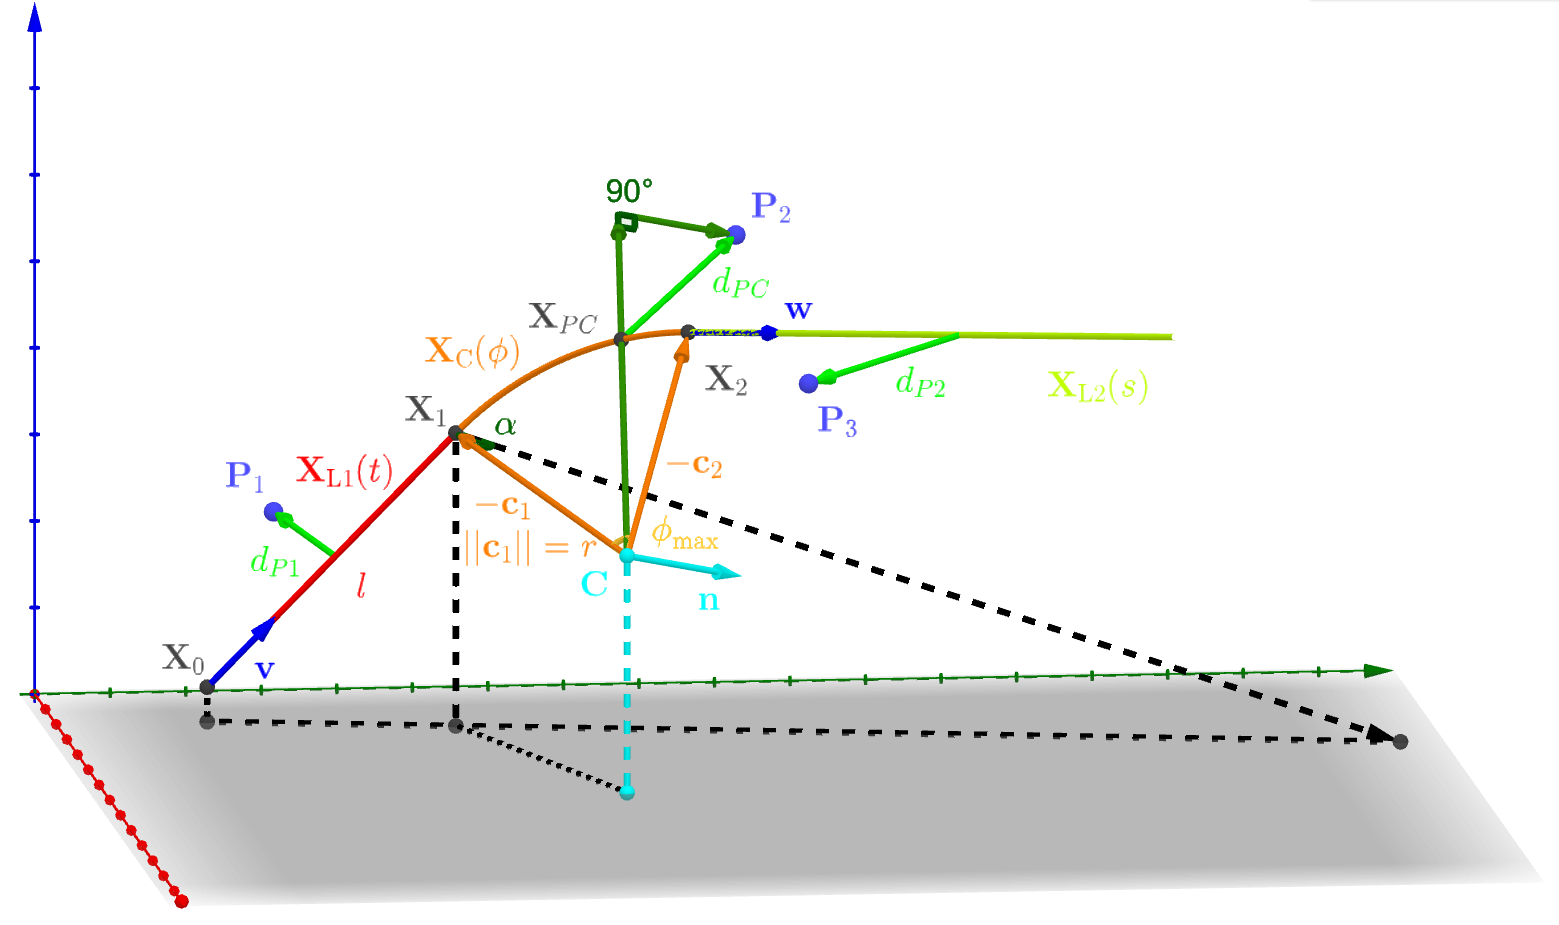
\includegraphics[width=\textwidth]{circle3d.png}
				\caption{Visualization of the 3D geometry of the circle-and-lines fit and its parameters. Projection of some points on the XY plane is shown to better display the spatial arrangement. Made with GeoGebra®.}
				\label{fig:circle3d}
			\end{figure}
			Using these parameters, we can derive a~parametrization of the whole curve. Let $\mathbf{v}$ be the initial unit direction vector, i.e., using the spherical angles
				\begin{equation}
					\mathbf{v} = (\cos\varphi\cos\theta, \,\sin\varphi\cos\theta, \,\sin\theta)^\mathrm{T},
				\end{equation}
			then we can parameterize the first line as follows:
				\begin{equation}
					\mathbf{X}_\text{L1}(t) = \mathbf{X}_0 + t\mathbf{v} \quad t\in[0,l].
				\end{equation}
			This gives us the starting point of the arc
				\begin{equation}
					\mathbf{X}_1 = \mathbf{X}_\text{L1}(l) = \mathbf{X}_0 + l\mathbf{v}.
				\end{equation}
			The vector $\mathbf{c}_1$ that lies in the plane of curvature and points from $\mathbf{X}_1$ to the center of curvature can be calculated using a~composition of rotations. First, we rotate $\mathbf{v}$ to point in the $\mathbf{\hat{x}}$ direction, the normal for $\alpha = 0$ than points in the $-\mathbf{\hat{z}}$ direction, we apply the $\alpha$ rotation and reverse the rotations into the $\mathbf{\hat{x}}$ direction:
				\begin{equation}
					\begin{aligned}
						\mathbf{c}_1 &= R_z(\varphi)R_y(-\theta)R_x(\alpha)R_y\left(\frac{\pi}{2}\right)R_y(\theta)R_z(-\varphi)\mathbf{v},\\
						&= R_z(\varphi)R_y(-\theta)R_x(\alpha)(-\mathbf{\hat{z}}),\\
						&= \scalebox{0.95}{$
								\begin{pmatrix}
									\cos\varphi & -\sin\varphi & 0\\
									\sin\varphi & \cos\varphi & 0\\
									0 & 0 & 1
								\end{pmatrix}
								\begin{pmatrix}
									\cos\theta & 0 & -\sin\theta\\
									0 & 1 & 0\\
									\sin\theta & 0 & \cos\theta
								\end{pmatrix}
								\begin{pmatrix}
									1 & 0 & 0\\
									0 & \cos\alpha & -\sin\alpha\\
									0 & \sin\alpha & \cos\alpha
								\end{pmatrix}
								\begin{pmatrix}
									0\\ 0\\ -1
								\end{pmatrix}
							$},\\
						&= 	\begin{pmatrix}
								-\sin\alpha\sin\varphi+\cos\alpha\cos\varphi\sin\theta\\
								\phantom{-}\sin\alpha\cos\varphi+\cos\alpha\sin\varphi\sin\theta\\
								-\cos\alpha\cos\theta
							\end{pmatrix}.
					\end{aligned}
				\end{equation}
			Similarly by rotating $\mathbf{\hat{y}}$, we can get the normal vector $\mathbf{n}=\mathbf{v}\cross\mathbf{c}_1$ perpendicular to the plane of the trajectory:
				\begin{equation}
					\mathbf{n} = R_z(\varphi)R_y(-\theta)R_x(\alpha)\mathbf{\hat{y}}=
									\begin{pmatrix}
										-\cos\alpha\sin\varphi-\sin\alpha\cos\varphi\sin\theta\\
										\phantom{-}\cos\alpha\cos\varphi-\sin\alpha\sin\varphi\sin\theta\\
										\sin\alpha\cos\theta
									\end{pmatrix}.
				\end{equation}
			This allows us to express the coordinates of the center $\mathbf{C}$ of the circular arc:
				\begin{equation}
					\mathbf{C} = \mathbf{X}_1+r\mathbf{c}_1.
				\end{equation}
			We can then get the parametrization and the endpoint of the circular arc using Rodrigues' rotation formula:
				\begin{gather}
					\begin{aligned}
						\mathbf{c}_2 &= \mathbf{c}_1\cos\phi_\text{max} + (\mathbf{n}\cross\mathbf{c}_1)\sin\phi_\text{max} + \mathbf{n}(\mathbf{n}\cdot\mathbf{c}_1)(1-\cos\phi_\text{max}),\\
						&= \mathbf{c}_1\cos\phi_\text{max} - \mathbf{v}\sin\phi_\text{max},
					\end{aligned}\\
					\mathbf{X}_\text{C}(\phi) = \mathbf{C} - r(\mathbf{c}_1\cos\phi - \mathbf{v}\sin\phi) \quad \phi\in[0,\phi_\text{max}],\\
					\mathbf{X}_2 = \mathbf{X}_\text{C}(\phi_\text{max}) = \mathbf{C} - r\mathbf{c}_2,
				\end{gather}
			and if we define the direction vector of the second line, we also get its parametrization
				\begin{gather}
					\mathbf{w} = \mathbf{v}\cos\phi_\text{max} + (\mathbf{n}\cross\mathbf{v})\sin\phi_\text{max} = \mathbf{v}\cos\phi_\text{max} + \mathbf{c}_1\sin\phi_\text{max},\\
					\mathbf{X}_\text{L2}(s) = \mathbf{X}_2 + s\mathbf{w} \quad s\in[0,\infty).
				\end{gather}
				
			The fit is performed as a~(weighted) least square minimization using the MIGRAD algorithm provided by the \texttt{TVirtualFitter} class in ROOT. We need to derive the distance of any point~$\mathbf{P}$ to the fitted curve. For the first line, we simply compute the parameter value of the closest point on the line:
				\begin{equation}
					\label{eq:segdist}
					\begin{aligned}
						t_\mathbf{P} &= \mathbf{v}\cdot(\mathbf{P}-\mathbf{X}_1),\\
						d_{\mathbf{P}1} &= \norm{\mathbf{P}-\mathbf{X}_\text{L1}(t_\mathbf{P})}.
					\end{aligned}
				\end{equation}
			If the parameter value is outside of its bounds defined above, we take the boundary value instead. The distance to the second line is computed likewise. For the circular arc, we find the closest point by projecting the center connecting line onto the arc plane:
				\begin{gather}
					\mathbf{X}_{PC} = \mathbf{C} + r\frac{(\mathbf{P}-\mathbf{C})-(\mathbf{n}\cdot(\mathbf{P}-\mathbf{C}))\mathbf{n}}{\norm{(\mathbf{P}-\mathbf{C})-(\mathbf{n}\cdot(\mathbf{P}-\mathbf{C}))\mathbf{n}}},\\
					d_{\mathbf{P}C} = \norm{\mathbf{P}-\mathbf{X}_{\mathbf{P}C}}
				\end{gather}
			If the point $\mathbf{X}_{\mathbf{P}C}$ lies outside of the arc, distance to the closest endpoint is taken instead\footnote{In some cases, the distance might be underestimated when the point is closer to the circle, the arc is a~part of, than to the curve. We have attempted to fix this issue, but for an unknown reason, it led to problems with the fit convergence.}. The shortest distance out of $d_{\mathbf{P}1},d_{\mathbf{P}C},d_{\mathbf{P}2}$ is then taken as the distance to the curve.
			
			For the calculation of the kinetic energy from the radius, we implemented two variants:
				\begin{enumerate}[nosep]
				 	\item the "middle field" method, using the perpendicular projection to the plane of the trajectory of magnetic field at a~point, where the circular arc crosses the central plane of the \ac{OFTPC} (parallel to the YZ plane), and
				 	\item the "average field" method using the average value of this projection along the circular arc.
				\end{enumerate}
			This way, we get two energy estimates $E_{\text{reco}}^{\text{mid}}$ and $E_{\text{reco}}^{\text{avg}}$. If needed, this choice can be further optimized, however, since this method will only provide an initial guess of the kinetic energy for the more sophisticated, and computationally heavy Runge-Kutta fit, it is not necessary to reach the best precision, and fast solutions are preferred.
			
			An example of a~fitted track (both the actual initial points and the discrete reconstruction of the track) from the microscopic grid-like testing sample (described in \cref{sec:microgrid}) is shown in \cref{fig:cfit3d}, the fitted parameters are given in \cref{tab:cfit3d}.
			
			\begin{table}
				\centering
				{\renewcommand{\arraystretch}{1.2}
					\begin{tabular}{|c|c|c|}
						\hline
						\textbf{Parameter} & \textbf{Fit of microscopic track} & \textbf{Fit of reconstructed track} \\
						\hline
						$l$ & \qty{-0.27 \pm 0.90}{\cm} & \qty{-0.26 \pm 0.62}{\cm} \\ \hline
						$\alpha$ & \qty{-6.2 \pm 2.3}{\degree} & \qty{-8.2 \pm 2.3}{\degree} \\ \hline
						$r$ & \qty{17.2 \pm 4.8}{\cm} & \qty{16.8 \pm 2.8}{\cm} \\ \hline
						$\phi_{\text{max}}$ & \qty{26.1 \pm 7.2}{\degree} & \qty{20.5 \pm 3.6}{\degree} \\ \hline
						$E_{\text{reco}}^{\text{mid}}$ & \qty{7.93}{\MeV} & \qty{7.35}{\MeV} \\ \hline
						$E_{\text{reco}}^{\text{avg}}$ & \qty{7.80}{\MeV} & \qty{8.19}{\MeV} \\ \hline
				\end{tabular}}
				\caption{3D circle fit parameters of an~\qty{8}{\MeV} track from the grid-like testing sample (described in \cref{sec:microgrid}) with minimal values of $\theta$ and $\phi$ initial direction angles.}
				\label{tab:cfit3d}
			\end{table}
			
			\begin{figure}
				\centering
				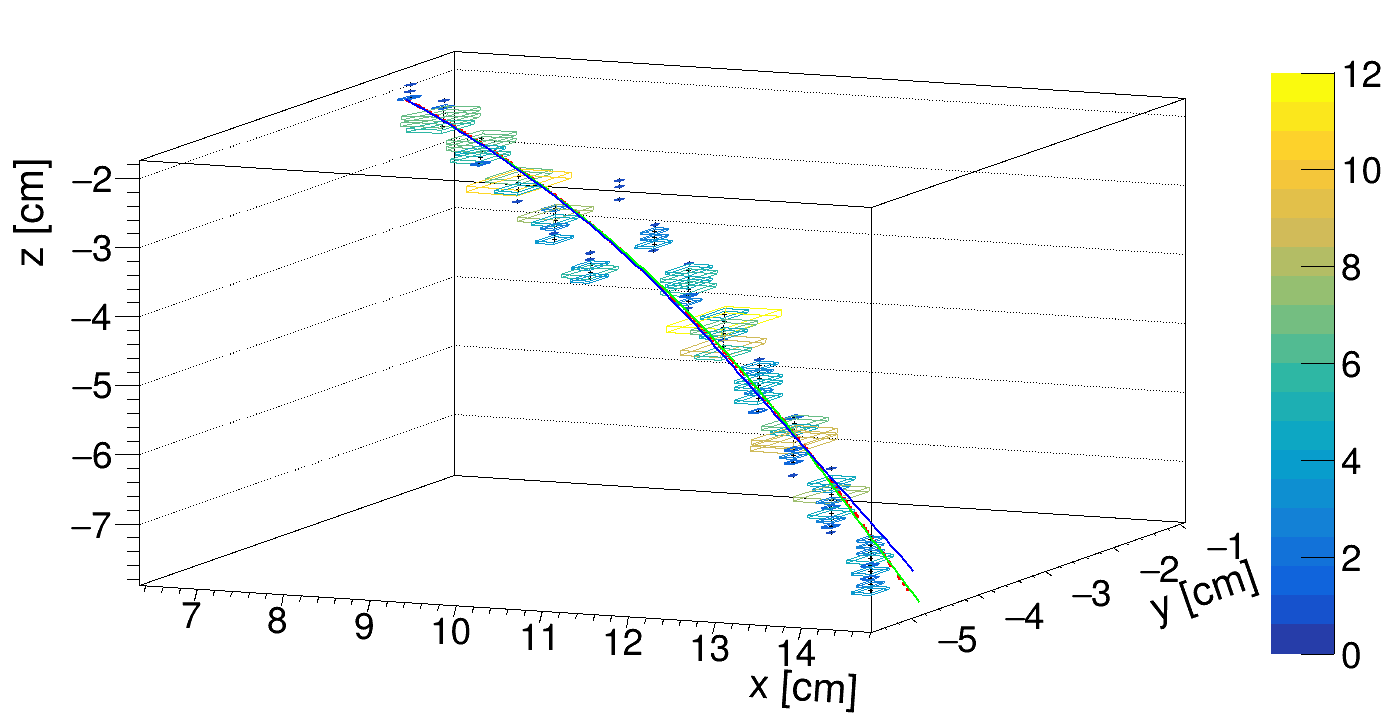
\includegraphics[width=\textwidth]{cfit3d_track.png}
				\caption{3D circle fit of an~\qty{8}{\MeV} track (red points) from the grid-like testing sample (described in \cref{sec:microgrid}) with minimal values of $\theta$ and $\phi$ initial direction angles. Both fits of the original (green) and reconstructed track (blue) are shown. Resulting parameter values are given in \cref{tab:cfit3d}.}
				\label{fig:cfit3d}
			\end{figure}			
			
			\subsection{Testing on a~Runge-Kutta sample}
				The three dimensional circle-and-lines fit was tested on a~sample of Runge-Kutta tracks with randomized parameters described in \cref{sec:rktest}. These tracks of primary electrons and positrons consist of points calculated with the \ac{RK4} algorithm for a~given time step. The parameter ranges in the MIGRAD minimizer have to be carefully tuned, simple exclusion of pathologic values can lead to convergence towards an edge value. After the tuning, only \num{4163} out of \num{1000000} tracks failed to converge to energy within \qty{2}{\MeV} from the simulation. We compared the two methods of choosing the magnetic fields. The resulting relative errors of reconstructed energy are shown in \cref{fig:cfit_rk}. When appropriate, we use the Freedman-Diaconis rule\footnote{The Freedman-Diaconis rule is equivalent to the Scott's rule for normally distributed data, but it uses the interquartile range instead of the sample standard deviation, which makes it less sensitive to outliers.} for bin width selection~\cite{FreedmanDiac}.

				We see that the average field method systematically underestimates the particle's energy, but has \textapprox25 times lower \acs{FWHM} (only \qty{0.77}{\percent}) than the average field method. This shows that, when corrected, this method can serve as a~good initial estimate of the particle's energy, before it gets refined by the Runge-Kutta fit.
				
				\begin{figure}
					\centering
					\begin{subfigure}[t]{\textwidth}
						\centering
						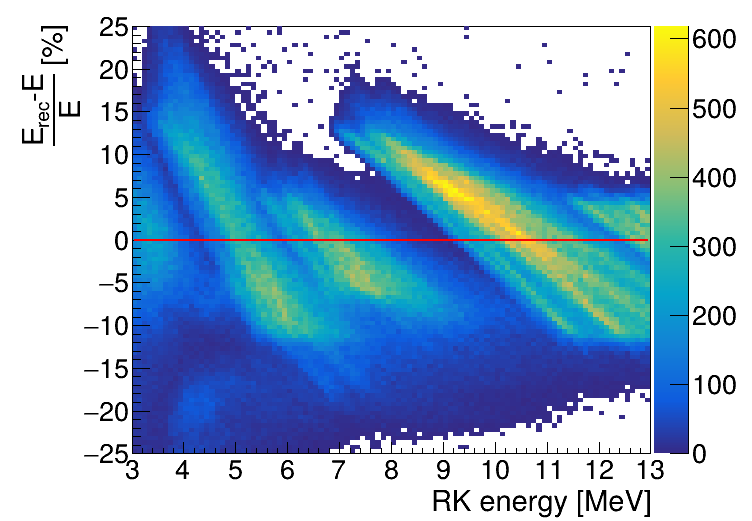
\includegraphics[width=0.48\textwidth]{cfit_diff_energy_mid.png}
						\hfill
						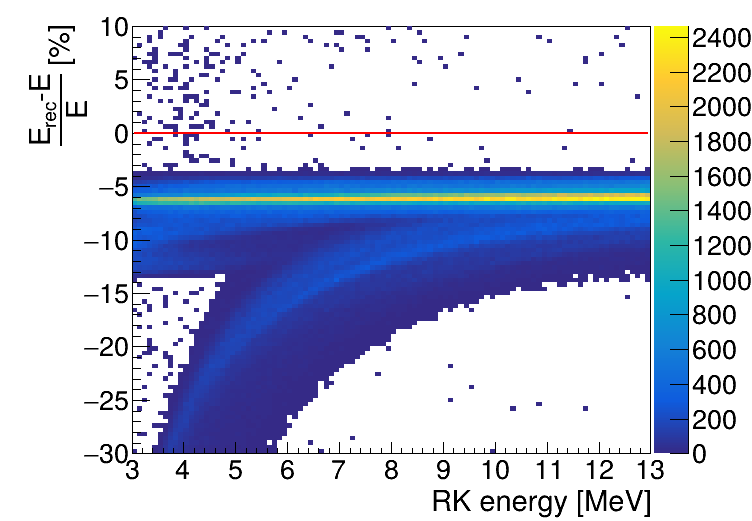
\includegraphics[width=0.48\textwidth]{cfit_diff_energy_avg.png}
						\caption{Dependence of relative error on simulated energy for both magnetic field selection methods.}
					\end{subfigure}
					\begin{subfigure}[t]{\textwidth}
						\centering
						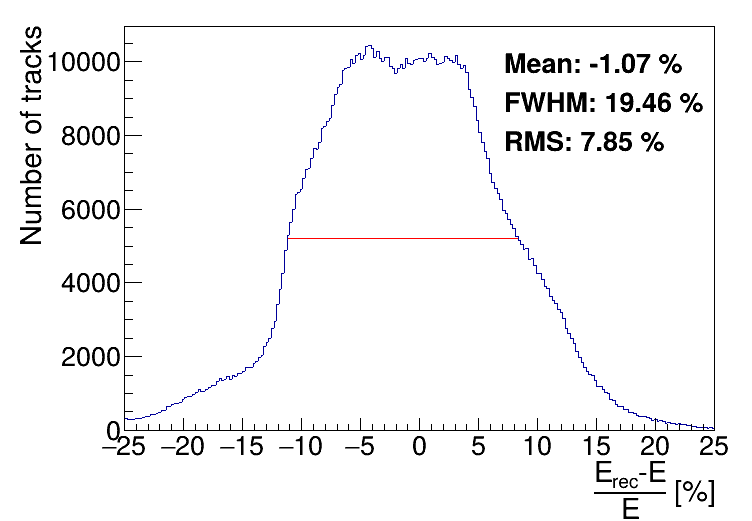
\includegraphics[width=0.48\textwidth]{cfit_diff_mid.png}
						\hfill
						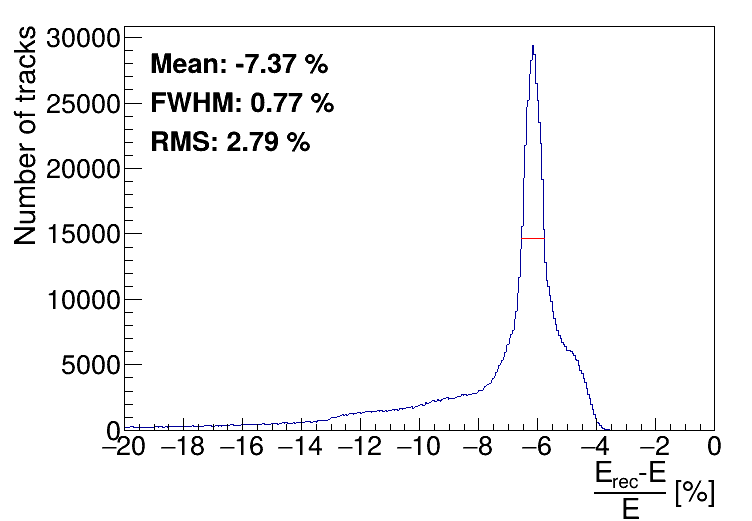
\includegraphics[width=0.48\textwidth]{cfit_diff_avg.png}
						\caption{Overall relative error for both magnetic field selection methods. Freedman-Diaconis rule was used for bin width selection.}
					\end{subfigure}
					\caption{Relative error of the energy of Runge-Kutta tracks reconstructed with the 3D circle-and-lines fit. The middle (left) and the average field (right) methods are compared. Dependence on the initial direction angles $\theta$ and $\varphi$ is small in comparison (for this reason, the plots are not shown).}
					\label{fig:cfit_rk}
				\end{figure}
	
	\section{Runge-Kutta Fit}
	\label{sec:rkfit}
		The Runge-Kutta fit uses the \acf{RK4} numerical integration of the equation of motion (see \cref{sec:rks}) to find the best values of the track parameters -- the track origin, initial velocity direction and the kinetic energy. In order to speed up the energy reconstruction, an initial guess of these parameters can be obtained from the 3D circle fit described in the previous section. Furthermore, assuming we know the track origin and orientation, we can perform a~single parameter fit of the kinetic energy.
		
		The fit is performed as a~least square minimization of the (weighted) distances of the track points (true ionization vertices from the simulation or reconstructed points). The simulated \ac{RK4}~track consists of line segments with known endpoints, therefore we can calculate the distance of a~point from this segment analogically to \cref{eq:segdist} with $\mathbf{v}$ given as a~unit vector in the direction of the segment.
		
		We need to find the segment with the lowest distance. We assume, that the distance $d_\mathbf{P}(\tau)$ of a~point $\mathbf{P}$ to the point on the track (a~curve parameterized by the proper time $\tau$) $\mathbf{X}(\tau)$ has a~single minimum (local and global), no local maximum (except the interval endpoints) and no~saddle point
			\begin{equation}
				\label{eq:rk_assum}
				\exists!\tau_\text{min}\in[0,\tau_N]\colon\ \left(\forall\tau\in[0,\tau_N]\colon  d_{\mathbf{P}}(\tau) \geq d_{\mathbf{P}}(\tau_\text{min})\right)\ \lor\ \dv{d_{\mathbf{P}}}{\tau}{(\tau_\text{min})} = 0,
			\end{equation}
		where $N$ is the number of \ac{RK4} steps. This is a~reasonable assumption for a~track with an approximate shape of a~circular arc with a~radius $r$, since the distance $d$ from a~point $\mathbf{C}$ on the corresponding circle of a~point $\mathbf{P}$ offset by~$a$ from the arc plane and by~$b$ from the arc's center when projected on its plane is given by the law of cosines:
			\begin{equation}
				\label{eq:rkdemo}
				d^2 = a^2+b^2+r^2 - 2br\cos\alpha,
			\end{equation}
		where $\alpha$ is the angle between points~$\mathbf{C}$ and~$\mathbf{P}$ as seen from the center of the arc (see \cref{fig:rkdemo}). This function is strictly convex for $\alpha\in\left(-\frac{\pi}{2},\frac{\pi}{2}\right)$ and in our case, the center of the arc lies outside of the detector and $\alpha$ is restricted to a~small interval around zero (especially considering that the initial guess should make the fitted trajectory reasonably close to any relevant point, in the worst-case scenario, the distance is overestimated, which should keep the fit from converging to such solutions).
		
		\begin{figure}
			\centering
			\begin{subfigure}[t]{0.7\textwidth}
				\centering
				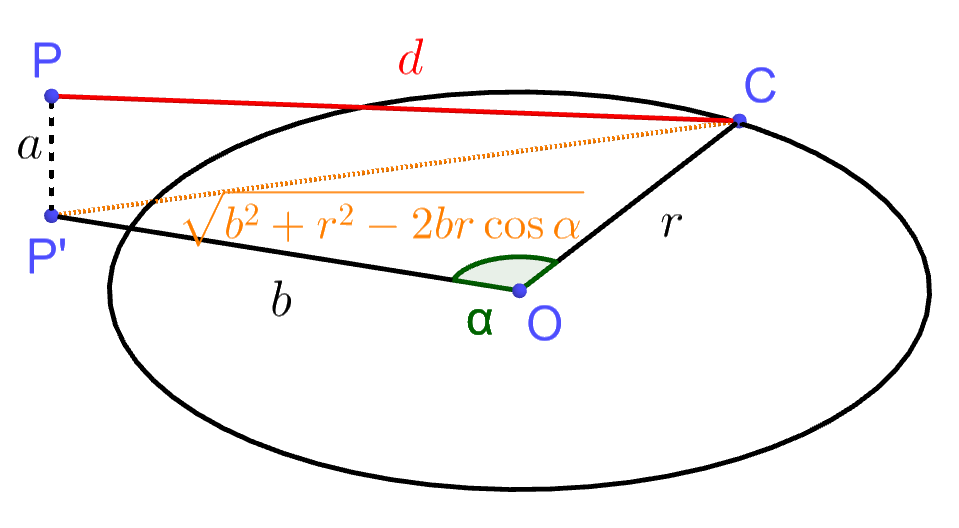
\includegraphics[width=\textwidth]{rk_circle_demo.png}
			\end{subfigure}
			\hfill
			\begin{subfigure}[t]{0.29\textwidth}
				\centering
				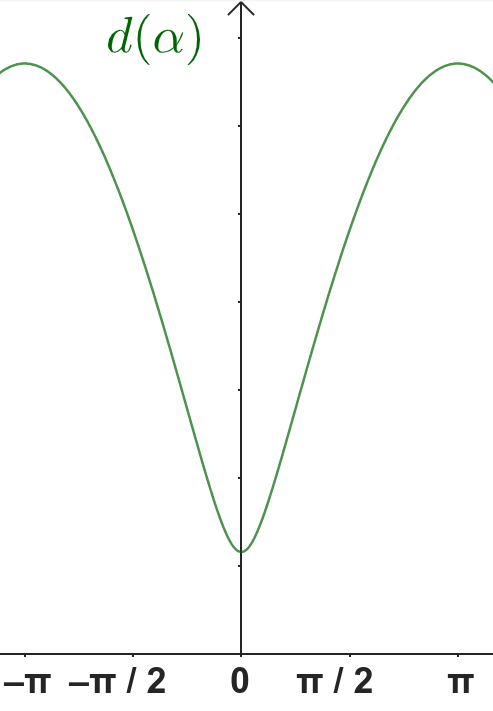
\includegraphics[width=\textwidth]{rk_circle_demo2.png}
			\end{subfigure}
			\caption{Demonstration of the convexity of the distance function $d(\alpha)$ for a~circular track (see \cref{eq:rkdemo}). Made with GeoGebra®.}
			\label{fig:rkdemo}
		\end{figure}
		
		In a~more general case, if we consider the vector $\mathbf{a}(\tau) = \mathbf{P}-\mathbf{X}(\tau)$ whose size is $\norm{\mathbf{a}(\tau)} = d_\mathbf{P}(\tau)$, then the we get
			\begin{equation}
				2d_{\mathbf{P}}\dv{d_{\mathbf{P}}}{\tau}= \dv{d^2_{\mathbf{P}}}{\tau} = 2\mathbf{a}\cdot\dv{\mathbf{a}}{\tau} = -2\mathbf{a}\cdot\dv{\mathbf{X}}{\tau},
			\end{equation}
		therefore for the derivative of~$d_\mathbf{P}(\tau)$ to be zero, $\mathbf{a}(\tau)$ has to be perpendicular to the tangent of the track. In 3D, for a~given $\mathbf{X}(\tau)$, this condition restricts $\mathbf{P}$ to a~plane. This means that on a~curving track, for any two points $\mathbf{X}(\tau_1),\mathbf{X}(\tau_2)$ with non-parallel tangents, we can find a~point~$\mathbf{P}$ that has $\dv{d_{\mathbf{P}}}{\tau}{(\tau_1)} = \dv{d_{\mathbf{P}}}{\tau}{(\tau_2)} = 0$, which violates the assumption~\ref{eq:rk_assum}. If we have a~circle-and-lines track as described in the previous sections, such a~point has to lie outside of the circular sector given by the arc.
		
		For a~planar track $\mathbf{X}(\tau) = \left(X_1(\tau),X_2(\tau)\right)$, the envelope of all its normals is the evolute of the curve (i.e., the set of centers of all its osculating circles). If the track has a~monotonous tangent angle
			\begin{equation}
				\alpha(\tau) = \atan{\frac{\dv{X_2}{\tau}}{\dv{X_1}{\tau}}}
			\end{equation}
		with minimal and maximal $\alpha$ differing by less than $\pi$ (i.e., the track changes direction by less than $180^\circ$), then all intersections of the track's normals must lie in an area bordered by the evolute and the normals at the beginning and the end of the curve (from their intersection with the evolute to their mutual intersection, see \cref{fig:rkdemo2,fig:rkdemo3}). Together, these three boundaries define a~closed shape that will lie outside of the \ac{OFTPC} for a~typical track in our detector\footnote{The smallest anticipated radius of curvature is \qty{39}{\cm} for an electron or positron with a~kinetic energy \qty{3}{\MeV} in a~\qty{0.3}{\tesla} magnetic field. All points in the exclusion area must be farther from the track and therefore outside the \ac{OFTPC}.}.
			\begin{figure}
				\centering
				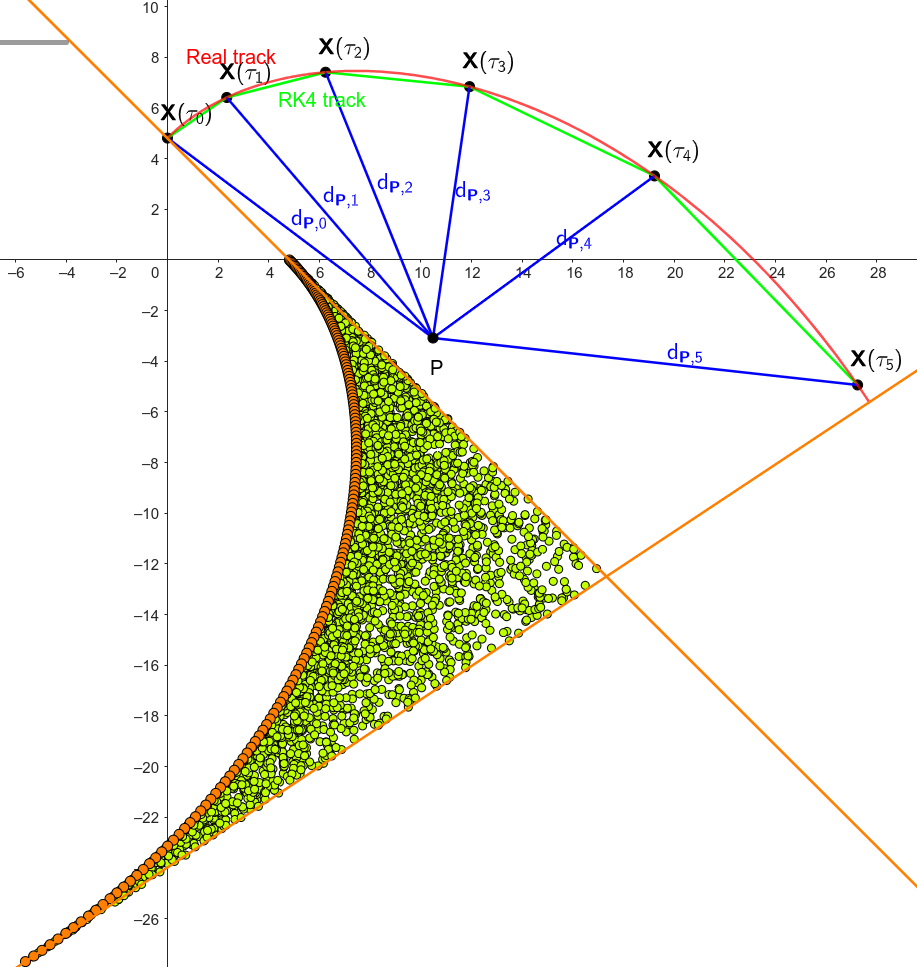
\includegraphics[width=0.55\textwidth]{rk_dist_demo.png}
				\hfill
				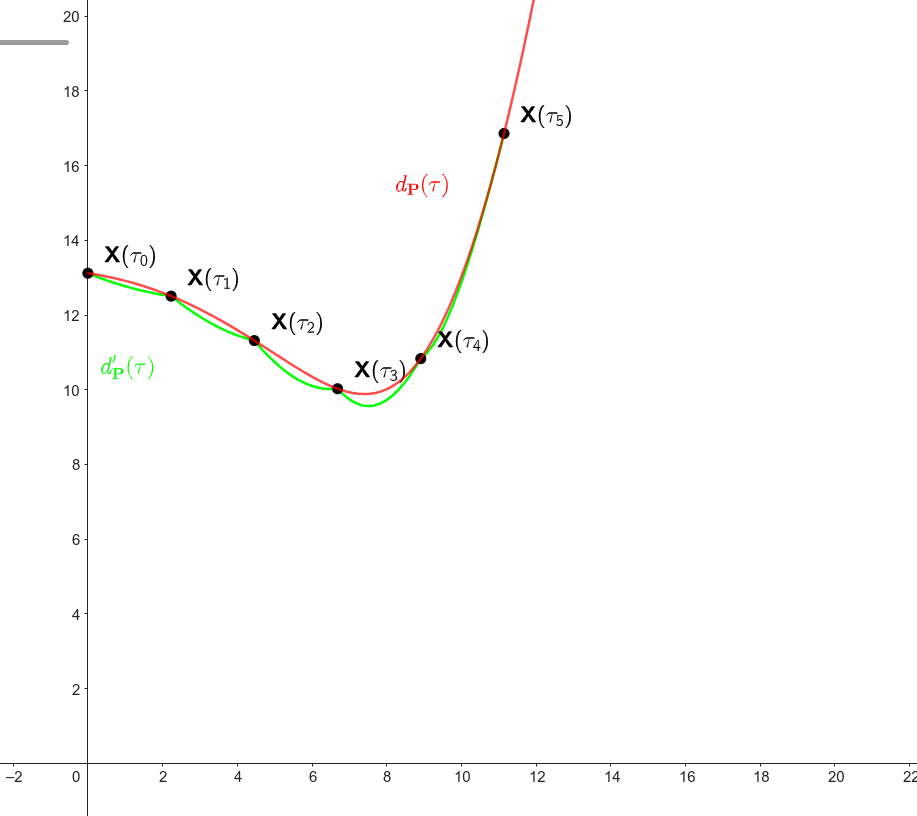
\includegraphics[width=0.42\textwidth]{rk_dist_demo2.png}
				\caption{An example track (red) with a~polygonal chain approximation (green, representing a~\ac{RK4} simulation). The distance of the point~$\mathbf{P}$ from the chain is found using a~binary search among the distances to the vertices $d_\mathbf{P}(\tau_i)$ (blue) and subsequently calculating the distance to segments neighboring the found vertex (thus finding the minimum of the function $d_\mathbf{P}'(\tau)$, function $d_\mathbf{P}(\tau)$ for the actual track is showed for reference). This approach works if the condition~\ref{eq:rk_assum} is satisfied, which is not the case for a~point from the green area bordered by the normals at endpoints and the evolute of the track (orange). Made with GeoGebra®.}
				\label{fig:rkdemo2}
			\end{figure}
			\begin{figure}
				\centering
				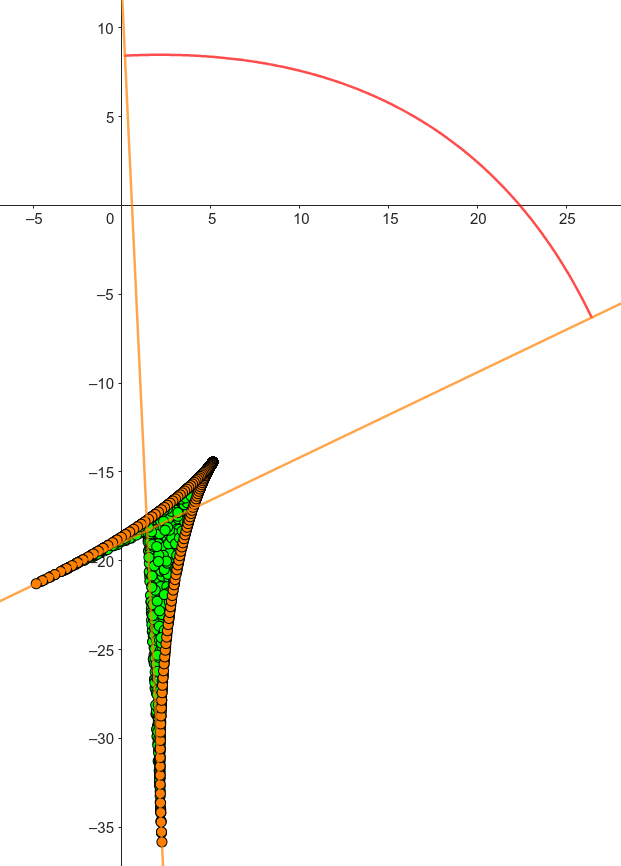
\includegraphics[width=0.6\textwidth]{rk_dist_demo3.png}
				\caption{An exclusion area (green) of a~track (red) bordered by its evolute and the normals at endpoints (orange), where the assumption~\ref{eq:rk_assum} is violated. Unlike the track in \cref{fig:rkdemo2}, this track has a~minimal curvature point in the middle, corresponding to the cusp on its evolute. Made with GeoGebra®.}
				\label{fig:rkdemo3}
			\end{figure}
		
		With the assumption~\ref{eq:rk_assum}, we can find the segment on the \ac{RK4} track with the lowest distance to a~given point~$\mathbf{P}$ using a~binary search algorithm. Let the distance of the point from the $n$\nobreakdash-th vertex %(resp. segment) 
		be~$d_{\mathbf{P},n} = d_{\mathbf{P}}(\tau_n)$%(resp.~$d_{\mathbf{P},n}'$). For every~$n$, there is a~$\tau_n'\in[\tau_{n-1},\tau_n]$ such that $d_{\mathbf{P}}(\tau_n') = d_{\mathbf{P},n}'$. Since~$d_{\mathbf{P}}(\tau)$ is a~continuous convex function and $\tau \in [0,\tau_N]$ for a~\ac{RK4} track with $N+1$~points, there is a~single minimum $d_{\textbf{P},\text{min}} = d_{\mathbf{P}}(\tau_\text{min})$ for some~$\tau_\text{min}\in[0,\tau_N]$%\in\{\tau_n'\}_{n=1}^N$.\footnote{the distance to two neighboring segments can be the same if the closest point is in their common vertex $\tau_n' = \tau_{n+1}'$}
		. Then the difference $\Delta d_{\mathbf{P},n} = d_{\mathbf{P},n}-d_{\mathbf{P},n-1}$ satisfies
			%\begin{equation}
			%	\begin{aligned}
			%		\Delta d_{\mathbf{P},n} &\leq 0\quad \forall n \in \{1,\ldots,k\},\\
			%		\Delta d_{\mathbf{P},n} &\geq 0\quad \forall n \in \{k+1,\ldots,N\}.
			%	\end{aligned}
			%\end{equation}
			\begin{equation}
				\begin{aligned}
					\Delta d_{\mathbf{P},n} &< 0\quad \forall n \text{ such that } \tau_n < \tau_\text{min},\\
					\Delta d_{\mathbf{P},n} &> 0\quad \forall n \text{ such that } \tau_{n-1} > \tau_\text{min}.
				\end{aligned}
			\end{equation}
		Therefore, we can search for the segment containing $d_{\textbf{P},\text{min}} = d_{\mathbf{P}}(\tau_\text{min})$ with binary search starting with $\Delta d_{\mathbf{P},1}$ and $\Delta d_{\mathbf{P},N}$, then calculate the difference $\Delta d_{\mathbf{P},m}$ for the middle index $m = \left\lfloor\frac{N+1}{2}\right\rfloor$. If $\Delta d_{\mathbf{P},m} > 0$, we can replace the higher index with~$m$, otherwise we replace the lower index. The search stops when the difference between the minimal and maximal index is one. The Fit itself is done using the MIGRAD algorithm implemented for the \texttt{TVirtualFitter} class in ROOT.
		
		\subsection{Testing on a~microscopic sample}
			The Runge-Kutta fit together with the 3D circle-and-lines pre-fit was tested on a~sample of tracks simulated using the microscopic simulation described in \cref{sec:microsim}. At first, few tracks with randomized initial parameters (same as the Runge-Kutta sample in \cref{sec:rktest}) were generated for preliminary testing. Later, a~sample with a~grid-like distribution of track parameters was generated (see \cref{sec:microgrid} for details). This allows us to test the performance of energy reconstruction from the microscopic tracks reconstructed with the discrete map inversion reconstruction.
			
			The dependence of the resulting relative differences of reconstructed Runge-Kutta versus simulated energy for electron and positron tracks are shown in \cref{fig:rk_dE_theta,fig:rk_dE_phi,fig:rk_dE_energy}, the overall resolution without corrections is shown in \cref{fig:rk_dE}. We can see that electrons, as well as tracks with high values of $\theta$, are reconstructed with a~higher precision thanks to the larger drift distance of ionization electrons, which results in their spreading across more readout channels (pads and time bins). The energy of electron tracks, especially for high energies, tends to be overestimated (and vice versa for positrons). This is related to the uncorrected shift in the map inversion $z$\nobreakdash-coordinate reconstruction as seen from the residuals in \cref{fig:7030_map_res}. This shift is caused by non-zero initial velocities of ionization electrons that is not accounted for by the map. It has opposite directions for electrons and positrons, because the ionization electrons are more likely to follow the direction of the ionizing particle, and it deforms the track, since it strengthens as the track curves. The effect is more pronounced for higher energies, where the curve is more sensitive to slight changes, as shown in \cref{fig:rk_forward}.

			\begin{figure}
				\centering
				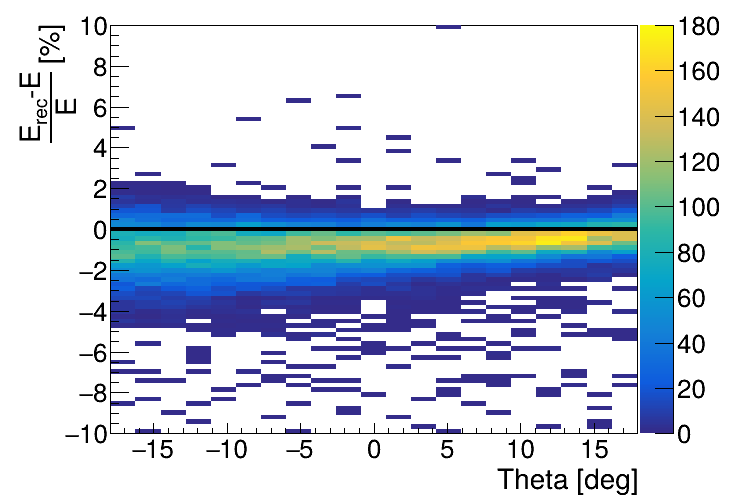
\includegraphics[width=0.48\textwidth]{rk_e_dE_th.png}
				\hfill
				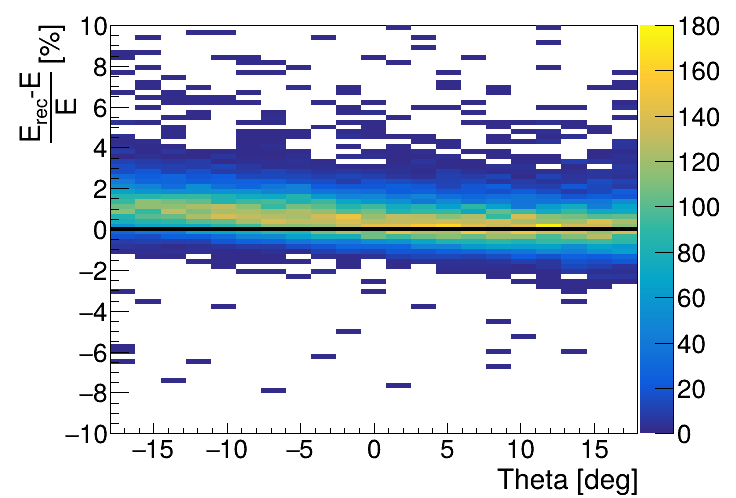
\includegraphics[width=0.48\textwidth]{rk_p_dE_th.png}
				\caption{Dependence on theta of relative differences of reconstructed Runge-Kutta versus simulated energy for the Runge-Kutta fit for electrons (left) and positrons (right).}
				\label{fig:rk_dE_theta}
			\end{figure}


			\begin{figure}
				\centering
				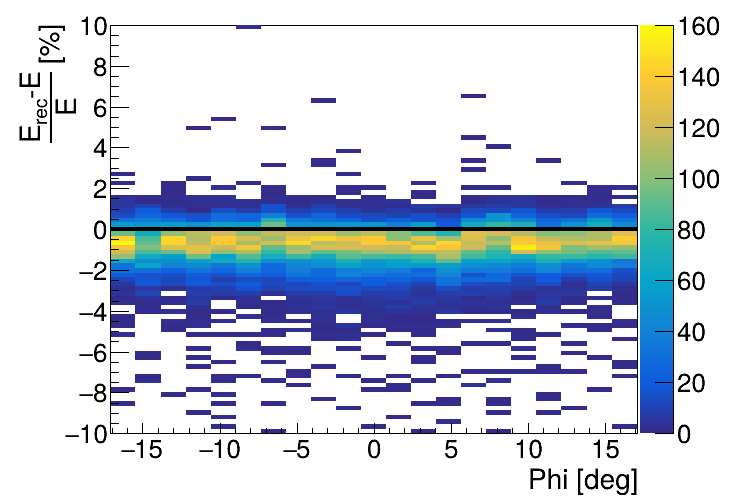
\includegraphics[width=0.48\textwidth]{rk_e_dE_ph.png}
				\hfill
				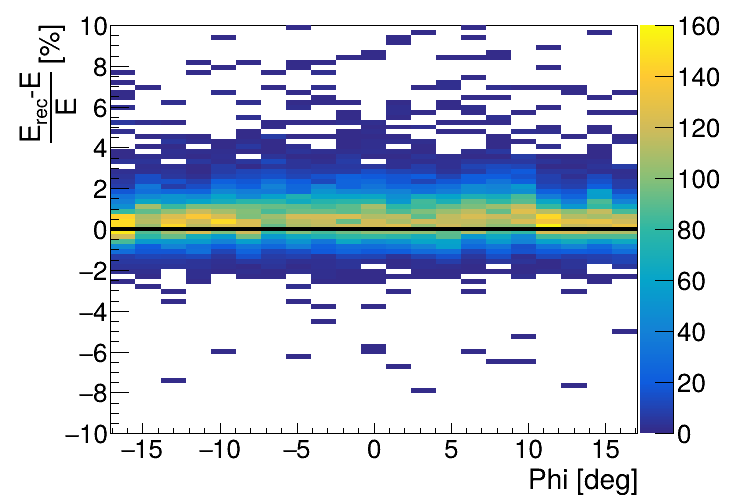
\includegraphics[width=0.48\textwidth]{rk_p_dE_ph.png}
				\caption{Dependence on theta of relative differences of reconstructed Runge-Kutta versus simulated energy for the Runge-Kutta fit for electrons (left) and positrons (right).}
				\label{fig:rk_dE_phi}
			\end{figure}

			\begin{figure}
				\centering
				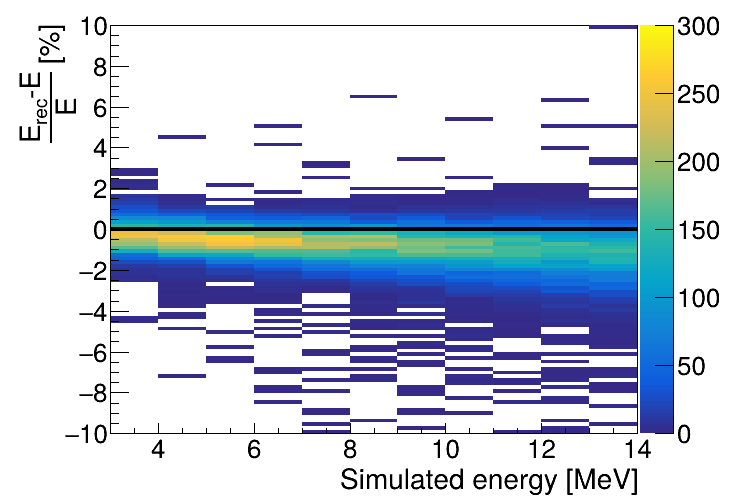
\includegraphics[width=0.48\textwidth]{rk_e_dE_E.png}
				\hfill
				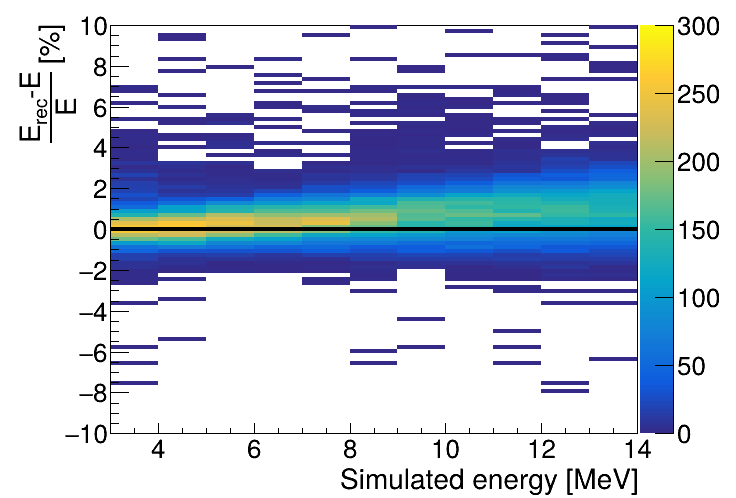
\includegraphics[width=0.48\textwidth]{rk_p_dE_E.png}
				\caption{Dependence on simulated energy of relative differences of reconstructed Runge-Kutta versus simulated energy for the Runge-Kutta fit for electrons (left) and positrons (right).}
				\label{fig:rk_dE_energy}
			\end{figure}

			\begin{figure}
				\centering
				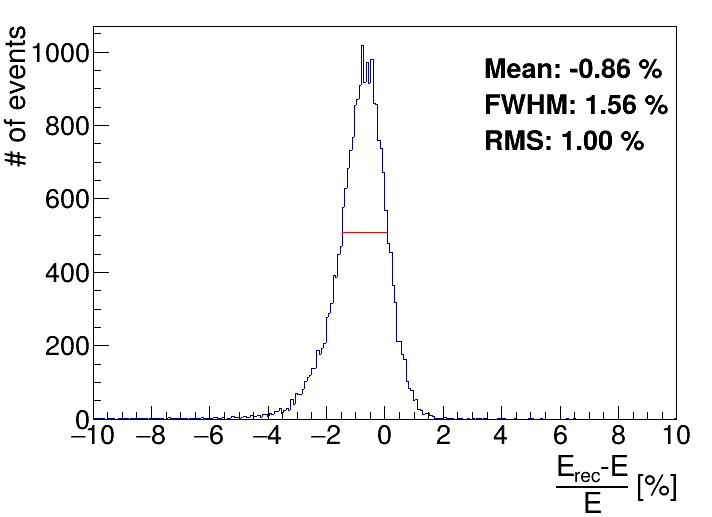
\includegraphics[width=0.48\textwidth]{rk_e_dE.png}
				\hfill
				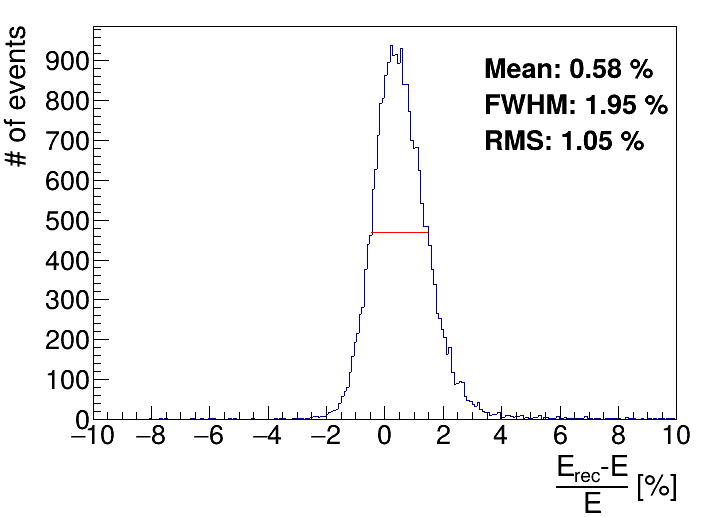
\includegraphics[width=0.48\textwidth]{rk_p_dE.png}
				\caption{The overall relative differences of reconstructed versus simulated energy for the Runge-Kutta fit for electrons (left) and positrons (right).}
				\label{fig:rk_dE}
			\end{figure}
			
			Since the Runge-Kutta fit is quite slow (each step of the MIGRAD algorithm has to simulate a~new track), we use the circle-and-lines fit to provide a~fast estimate, and to ensure the fit convergence. From \cref{fig:cfit_rk}, we see that the average field method offers the best estimate when corrected. We can again save both estimates from the circle-and-lines fit, this time measuring its performance on a~track reconstructed with discrete map inversion. The resulting histograms for electron and positron tracks are shown in \cref{fig:cfit_avg,fig:cfit_mid}. We again find that the average field method performs much better.
			
			\begin{figure}
				\centering
				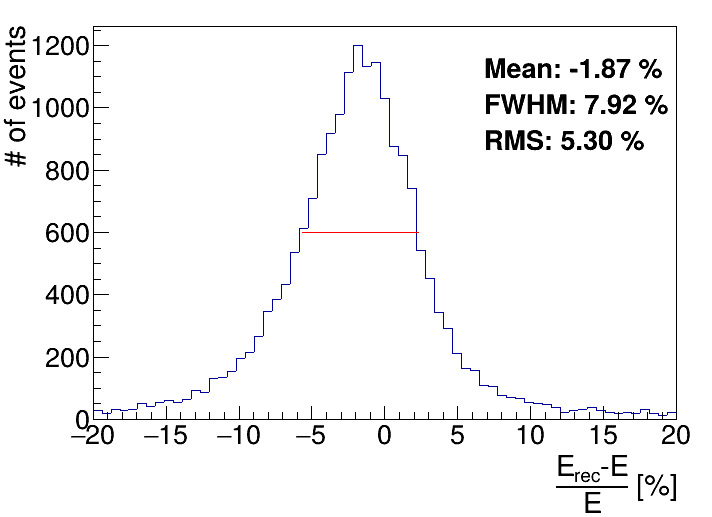
\includegraphics[width=0.48\textwidth]{cfit_avg_e_dE.png}
				\hfill
				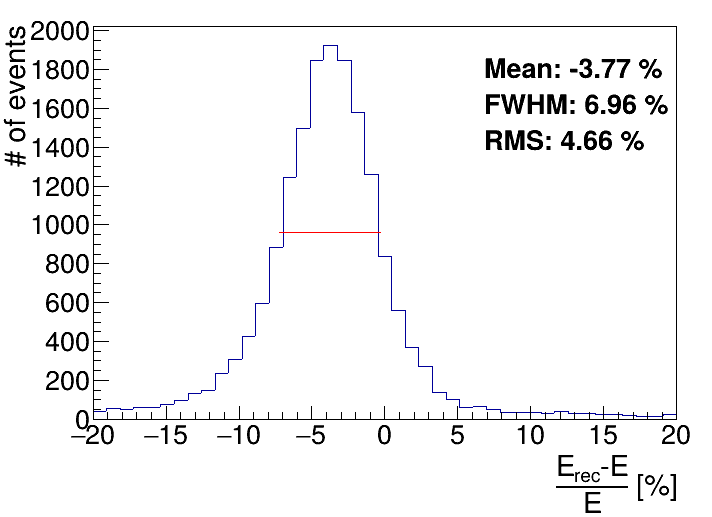
\includegraphics[width=0.48\textwidth]{cfit_avg_p_dE.png}
				\caption{The overall relative differences of reconstructed versus simulated energy for the circle-and-lines (average field, corrected) for electrons (left) and positrons (right).}
				\label{fig:cfit_avg}
			\end{figure}
			
			\begin{figure}
				\centering
				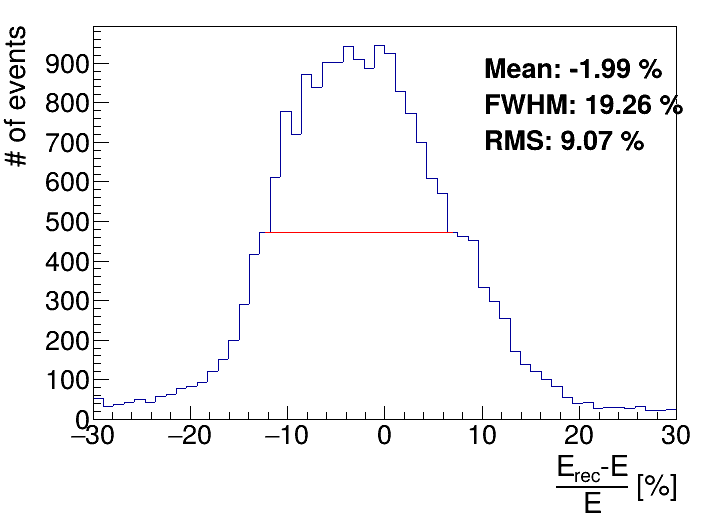
\includegraphics[width=0.48\textwidth]{cfit_mid_e_dE.png}
				\hfill
				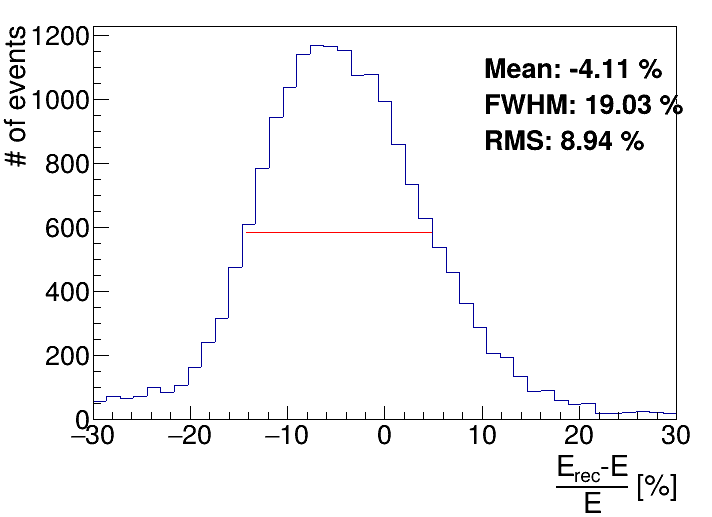
\includegraphics[width=0.48\textwidth]{cfit_mid_p_dE.png}
				\caption{The overall relative differences of reconstructed versus simulated energy for the circle-and-lines (middle field) for electrons (left) and positrons (right).}
				\label{fig:cfit_mid}
			\end{figure}